\documentclass[UTF8,12pt]{ctexart}
\usepackage{amsmath,amssymb,geometry,bm,graphicx,fontspec,amssymb,amsthm}
\usepackage[mathscr]{euscript}
\usepackage{array}

\usepackage[colorlinks,
linkcolor=black,
anchorcolor=blue,
citecolor=green
]{hyperref} % 目录中的超链接

\usepackage{tikz}
\usetikzlibrary{calc}
\usetikzlibrary{shapes.geometric}
% Node styles
\tikzset{
	% Two node styles for game trees: solid and hollow
	solid node/.style={circle,draw,inner sep=1.5,fill=black},
	hollow node/.style={circle,draw,inner sep=1.5}
}

\newtheorem{Def}{定义}[section]
\newtheorem{Theo}{定理}[section]
\newtheorem{Lemm}{引理}[section]
\newtheorem{Prop}{命题}[section]
\newtheorem{Axiom}{Axiom}

\numberwithin{equation}{section} % 按章节进行排序与编号
\numberwithin{figure}{section}
\numberwithin{table}{section}

\usepackage{draftwatermark} % 所有页加水印
\SetWatermarkText{EconNerd} % 设置水印内容
\SetWatermarkLightness{0.99} % 设置水印透明度 0-1
\SetWatermarkScale{1} % 设置水印大小    

\title{博弈论} % 文档相关信息
\author{EconNerd}
\date{\today}
\geometry{scale=0.8}

\begin{document}
	\maketitle
	
		\begin{figure}[thbp]
		\centering
		\begin{tikzpicture}[scale=0.9,font=\footnotesize,centered]
			% macro for inputing payoff vectors
			\newcommand{\payoff}[3][below]{\node[#1]at(#2){#3};}
			% Specify spacing for each level of the tree
			\tikzstyle{level 1}=[level distance=15mm,sibling distance=30mm]
			\tikzstyle{level 2}=[level distance=15mm,sibling distance=30mm]	
			\tikzstyle{level 3}=[level distance=15mm,sibling distance=30mm]	

				\node(0)[hollow node,label=above:{Prosecutor},label=below:{$x_0$}]{}
				child{node(0-1)[solid node,label = left:{$x_1$}]{}
					edge from parent[draw] node[left]{不指控}
				} 
				child{node(0-2)[solid node,label = right:{Defendant},label = left:{$x_2$}]{} 
					child{
						node(0-2-1)[solid node,label = left:{Prosecutor},label = right:{$x_3$}]{} 
						child{
							node(0-2-1-1)[solid node,label = left:{$x_5$}]{}
							edge from parent[draw] node[left]{起诉}
						}
						child{
							node(0-2-1-2)[solid node,label = left:{$x_6$}]{}
							edge from parent[draw] node[right]{放弃}
						}
						edge from parent[draw] node[left]{应诉}
					} 
					child{
						node(0-2-2)[solid node,label = left:{$x_4$}]{} 
						edge from parent[draw] node[right]{接受}
					} 
					edge from parent[draw] node[right]{指控}
				}
			;
			\payoff{0-1}{$(0,0)$}
			\payoff{0-2-2}{$(s-c,-s)$}
			\payoff{0-2-1-1}{$(\gamma X - c - p,-\gamma X - d)$}
			\payoff{0-2-1-2}{$(-c,0)$}
		\end{tikzpicture}
	\end{figure}

	\begin{figure}[thbp]
		\centering
		\begin{tikzpicture}[scale=0.9,font=\footnotesize,centered]
			% macro for inputing payoff vectors
			\newcommand{\payoff}[3][below]{\node[#1]at(#2){#3};}
			\newcommand{\assnum}[3][left]{\node[#1]at(#2){#3};}
			% Specify spacing for each level of the tree
			\tikzstyle{level 1}=[level distance=15mm,sibling distance=15mm]
			\tikzstyle{level 2}=[level distance=15mm,sibling distance=30mm]	
			\tikzstyle{level 3}=[level distance=15mm,sibling distance=30mm]	
			
			\node(0-0)[hollow node,label = left:{Prosecutor}]{}
			child{
				node(0)[solid node,label=left:{Prosecutor}]{}
				child{
					node(0-1)[solid node]{}
					edge from parent[draw] node[left]{不指控}
				} 
				child{
					node(0-2)[solid node,label = right:{Defendant}]{} 
					child{
						node(0-2-1)[solid node,label = left:{Prosecutor}]{} 
						child{
							node(0-2-1-1)[solid node]{}
							edge from parent[draw] node[left]{起诉}
						}
						child{
							node(0-2-1-2)[solid node]{}
							edge from parent[draw] node[right]{放弃}
						}
						edge from parent[draw] node[left]{应诉}
					} 
					child{
						node(0-2-2)[solid node]{} 
						edge from parent[draw] node[right]{接受}
					} 
					edge from parent[draw] node[right]{指控}
				}
				edge from parent[draw] node[right]{支出律师费$p$}
			}
			;
			\payoff{0-1}{$(-p,0)$}
			\payoff{0-2-2}{$(s-c-p,-s)$}
			\payoff{0-2-1-1}{$(\gamma X - c - p,-\gamma X - d)$}
			\payoff{0-2-1-2}{$(-c-p,0)$}
			
			\assnum[right]{0-0}{$x_0$}
			\assnum[right]{0}{$x_1$}
			\assnum{0-1}{$x_2$}
			\assnum{0-2}{$x_3$}
			\assnum[right]{0-2-1}{$x_4$}
			\assnum{0-2-2}{$x_5$}
			\assnum{0-2-1-1}{$x_6$}
			\assnum{0-2-1-2}{$x_7$}
		\end{tikzpicture}
	\end{figure}

	\begin{figure}[thbp]
		\centering
		\begin{tikzpicture}[scale=0.9,font=\footnotesize,centered]
			% macro for inputing payoff vectors
			\newcommand{\payoff}[3][below]{\node[#1]at(#2){#3};}
			\newcommand{\assnum}[3][left]{\node[#1]at(#2){$x_#3$};}
			% Specify spacing for each level of the tree
			\tikzstyle{level 1}=[level distance=15mm,sibling distance=15mm]
			\tikzstyle{level 2}=[level distance=15mm,sibling distance=30mm]	
			\tikzstyle{level 3}=[level distance=15mm,sibling distance=30mm]	
			
			\node(0-0-0)[hollow node,label = left:{Defendant}]{}
			child{
				node(0-0)[hollow node,label = left:{Prosecutor}]{}
				child{
					node(0)[solid node,label=left:{Prosecutor}]{}
					child{
						node(0-1)[solid node]{}
						edge from parent[draw] node[left]{不指控}
					} 
					child{
						node(0-2)[solid node,label = right:{Defendant}]{} 
						child{
							node(0-2-1)[solid node,label = left:{Prosecutor}]{} 
							child{
								node(0-2-1-1)[solid node]{}
								edge from parent[draw] node[left]{起诉}
							}
							child{
								node(0-2-1-2)[solid node]{}
								edge from parent[draw] node[right]{放弃}
							}
							edge from parent[draw] node[left]{应诉}
						} 
						child{
							node(0-2-2)[solid node]{} 
							edge from parent[draw] node[right]{接受}
						} 
						edge from parent[draw] node[right]{指控}
					}
					edge from parent[draw] node[right]{支出律师费$p$}
				}
				edge from parent[draw] node[right]{支出律师费$d_1$}
			}
			
			
			;
			\payoff{0-1}{$(-p,0)$}
			\payoff{0-2-2}{$(s-c-p,-s)$}
			\payoff{0-2-1-1}{$(\gamma X - c - p,-\gamma X - d)$}
			\payoff{0-2-1-2}{$(-c-p,0)$}
			
			\assnum[right]{0-0-0}{0}
			\assnum[right]{0-0}{1}
			\assnum[right]{0}{2}
			\assnum{0-1}{3}
			\assnum{0-2}{4}
			\assnum[right]{0-2-1}{5}
			\assnum{0-2-2}{6}
			\assnum{0-2-1-1}{7}
			\assnum{0-2-1-2}{8}
		\end{tikzpicture}
	\end{figure}
	\begin{figure}[thbp]
		\centering
		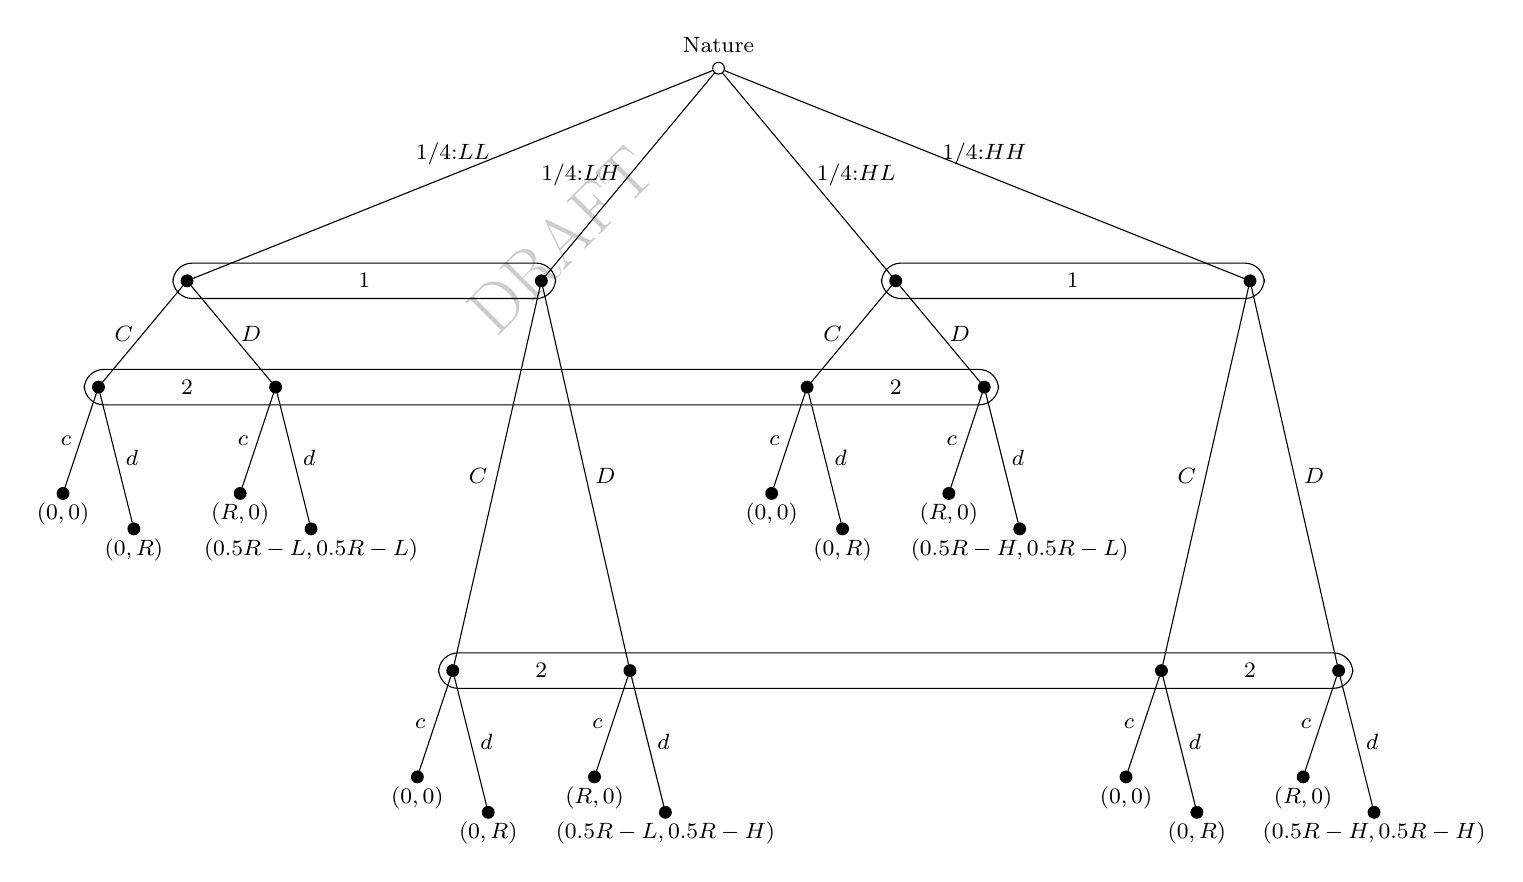
\begin{tikzpicture}[scale=0.9,font=\footnotesize,centered]
			% macro for inputing payoff vectors
			\newcommand{\payoff}[3][below]{\node[#1]at(#2){#3};}
			\newcommand{\assnum}[3][left]{\node[#1]at(#2){$x_#3$};}
			% Specify spacing for each level of the tree
			\tikzstyle{level 1}=[level distance=30mm,sibling distance=50mm]
			% \tikzstyle{level 2}=[level distance=15mm,sibling distance=30mm]	
			% \tikzstyle{level 3}=[level distance=15mm,sibling distance=30mm]	
			
			\node(0)[hollow node,label = above:{Nature}]{}
			child{
				node(0-1)[solid node]{}
				child[level distance=15mm,sibling distance=25mm]{
					node(0-1-1)[solid node]{}
					child[sibling distance=10mm]{
						node(0-1-1-1)[solid node]{}
						edge from parent[draw] node[left]{$c$}
					}
					child[level distance = 20mm,sibling distance=10mm]{
						node(0-1-1-2)[solid node]{}
						edge from parent[draw] node[right]{$d$}
					}
					edge from parent[draw] node[left]{$C$}
				}
				child[level distance=15mm,sibling distance=25mm]{
					node(0-1-2)[solid node]{}
					child[sibling distance=10mm]{
						node(0-1-2-1)[solid node]{}
						edge from parent[draw] node[left]{$c$}
					}
					child[level distance = 20mm,sibling distance=10mm]{
						node(0-1-2-2)[solid node]{}
						edge from parent[draw] node[right]{$d$}
					}
					edge from parent[draw] node[right]{$D$}
				}
				edge from parent[draw] node[above]{1/4:$LL$}
			}
			child{
				node(0-2)[solid node]{}
				child[level distance=55mm,sibling distance=25mm]{
					node(0-2-1)[solid node]{}
					child[level distance = 15mm,sibling distance=10mm]{
						node(0-2-1-1)[solid node]{}
						edge from parent[draw] node[left]{$c$}
					}
					child[level distance = 20mm,sibling distance=10mm]{
						node(0-2-1-2)[solid node]{}
						edge from parent[draw] node[right]{$d$}
					}
					edge from parent[draw] node[left]{$C$}
				}
				child[level distance=55mm,sibling distance=25mm]{
					node(0-2-2)[solid node]{}
					child[level distance = 15mm,sibling distance=10mm]{
						node(0-2-2-1)[solid node]{}
						edge from parent[draw] node[left]{$c$}
					}
					child[level distance = 20mm,sibling distance=10mm]{
						node(0-2-2-2)[solid node]{}
						edge from parent[draw] node[right]{$d$}
					}
					edge from parent[draw] node[right]{$D$}
				}
				edge from parent[draw] node[left]{1/4:$LH$}
			}
			child{
				node(0-3)[solid node]{}
				child[level distance=15mm,sibling distance=25mm]{
					node(0-3-1)[solid node]{}
					child[sibling distance=10mm]{
						node(0-3-1-1)[solid node]{}
						edge from parent[draw] node[left]{$c$}
					}
					child[level distance = 20mm,sibling distance=10mm]{
						node(0-3-1-2)[solid node]{}
						edge from parent[draw] node[right]{$d$}
					}
					edge from parent[draw] node[left]{$C$}
				}
				child[level distance=15mm,sibling distance=25mm]{
					node(0-3-2)[solid node]{}
					child[sibling distance=10mm]{
						node(0-3-2-1)[solid node]{}
						edge from parent[draw] node[left]{$c$}
					}
					child[level distance = 20mm,sibling distance=10mm]{
						node(0-3-2-2)[solid node]{}
						edge from parent[draw] node[right]{$d$}
					}
					edge from parent[draw] node[right]{$D$}
				}
				edge from parent[draw] node[right]{1/4:$HL$}
			}
			child{
				node(0-4)[solid node]{}
				child[level distance=55mm,sibling distance=25mm]{
					node(0-4-1)[solid node]{}
					child[level distance = 15mm,sibling distance=10mm]{
						node(0-4-1-1)[solid node]{}
						edge from parent[draw] node[left]{$c$}
					}
					child[level distance = 20mm,sibling distance=10mm]{
						node(0-4-1-2)[solid node]{}
						edge from parent[draw] node[right]{$d$}
					}
					edge from parent[draw] node[left]{$C$}
				}
				child[level distance=55mm,sibling distance=25mm]{
					node(0-4-2)[solid node]{}
					child[level distance = 15mm,sibling distance=10mm]{
						node(0-4-2-1)[solid node]{}
						edge from parent[draw] node[left]{$c$}
					}
					child[level distance = 20mm,sibling distance=10mm]{
						node(0-4-2-2)[solid node]{}
						edge from parent[draw] node[right]{$d$}
					}
					edge from parent[draw] node[right]{$D$}
				}
				edge from parent[draw] node[above]{1/4:$HH$}
			}
			;
			\payoff{0-1-1-1}{$(0,0)$}
			\payoff{0-1-1-2}{$(0,R)$}
			\payoff{0-1-2-1}{$(R,0)$}
			\payoff{0-1-2-2}{$(0.5R-L,0.5R-L)$}
			\payoff{0-2-1-1}{$(0,0)$}
			\payoff{0-2-1-2}{$(0,R)$}
			\payoff{0-2-2-1}{$(R,0)$}
			\payoff{0-2-2-2}{$(0.5R-L,0.5R-H)$}
			\payoff{0-3-1-1}{$(0,0)$}
			\payoff{0-3-1-2}{$(0,R)$}
			\payoff{0-3-2-1}{$(R,0)$}
			\payoff{0-3-2-2}{$(0.5R-H,0.5R-L)$}
			\payoff{0-4-1-1}{$(0,0)$}
			\payoff{0-4-1-2}{$(0,R)$}
			\payoff{0-4-2-1}{$(R,0)$}
			\payoff{0-4-2-2}{$(0.5R-H,0.5R-H)$}
			
			% information set
			\draw[rounded corners=7]($(0-1)+(-.2,.25)$)rectangle($(0-2)+(.2,-.25)$);
			\node at($(0-1)!.5!(0-2)$){1};
			
			\draw[rounded corners=7]($(0-3)+(-.2,.25)$)rectangle($(0-4)+(.2,-.25)$);
			\node at($(0-3)!.5!(0-4)$){1};
			
			\draw[rounded corners=7]($(0-1-1)+(-.2,.25)$)rectangle($(0-3-2)+(.2,-.25)$);
			\node at($(0-1-1)!.5!(0-1-2)$){2};
			\node at($(0-3-1)!.5!(0-3-2)$){2};
			
			\draw[rounded corners=7]($(0-2-1)+(-.2,.25)$)rectangle($(0-4-2)+(.2,-.25)$);
			\node at($(0-2-1)!.5!(0-2-2)$){2};
			\node at($(0-4-1)!.5!(0-4-2)$){2};
		\end{tikzpicture}
	\end{figure}

	\begin{figure}[thbp]
		\centering
		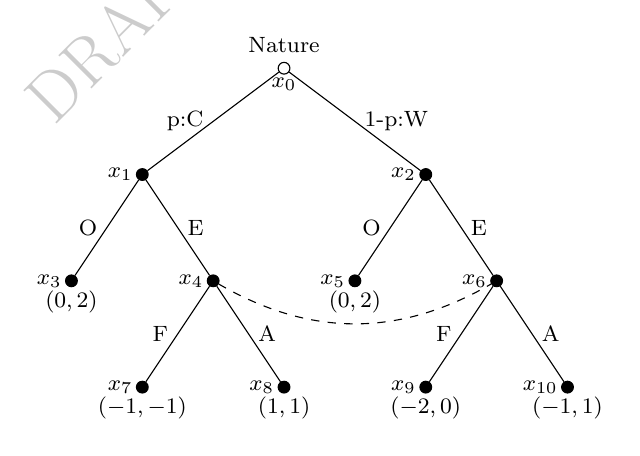
\begin{tikzpicture}[scale=0.9,font=\footnotesize,centered]
			% macro for inputing payoff vectors
			\newcommand{\payoff}[3][below]{\node[#1]at(#2){#3};}
			\newcommand{\assnum}[3][left]{\node[#1]at(#2){#3};}
			% Specify spacing for each level of the tree
			\tikzstyle{level 1}=[level distance=15mm,sibling distance=40mm]
			\tikzstyle{level 2}=[level distance=15mm,sibling distance=20mm]	
			\tikzstyle{level 3}=[level distance=15mm,sibling distance=20mm]	
			
			\node(0)[hollow node,label = above:{Nature}]{}
			child{
				node(0-1)[solid node]{}
				child{
					node(0-1-1)[solid node]{}
					edge from parent[draw] node[left]{O}
				}
				child{
					node(0-1-2)[solid node]{}
					child{
						node(0-1-2-1)[solid node]{}
						edge from parent[draw] node[left]{F}
					}
					child{
						node(0-1-2-2)[solid node]{}
						edge from parent[draw] node[right]{A}
					}
					edge from parent[draw] node[right]{E}
				}
				edge from parent[draw] node[left]{p:C}
			}
			child{
				node(0-2)[solid node]{}
				child{
					node(0-2-1)[solid node]{}
					edge from parent[draw] node[left]{O}
				}
				child{
					node(0-2-2)[solid node]{}
					child{
						node(0-2-2-1)[solid node]{}
						edge from parent[draw] node[left]{F}
					}
					child{
						node(0-2-2-2)[solid node]{}
						edge from parent[draw] node[right]{A}
					}
					edge from parent[draw] node[right]{E}
				}
				edge from parent[draw] node[right]{1-p:W}
			}
			;
			
			\assnum[below]{0}{$x_0$}
			\assnum{0-1}{$x_1$}
			\assnum{0-2}{$x_2$}
			\assnum{0-1-1}{$x_3$}
			\assnum{0-1-2}{$x_4$}
			\assnum{0-2-1}{$x_5$}
			\assnum{0-2-2}{$x_6$}
			\assnum{0-1-2-1}{$x_7$}
			\assnum{0-1-2-2}{$x_8$}
			\assnum{0-2-2-1}{$x_9$}
			\assnum{0-2-2-2}{$x_{10}$}
			
			\payoff{0-1-1}{$(0,2)$}
			\payoff{0-2-1}{$(0,2)$}
			\payoff{0-1-2-1}{$(-1,-1)$}
			\payoff{0-1-2-2}{$(1,1)$}
			\payoff{0-2-2-1}{$(-2,0)$}
			\payoff{0-2-2-2}{$(-1,1)$}
			
			\draw[dashed,bend right](0-1-2) to (0-2-2);
		\end{tikzpicture}
	\end{figure}

	\begin{figure}[thbp]
		\centering
		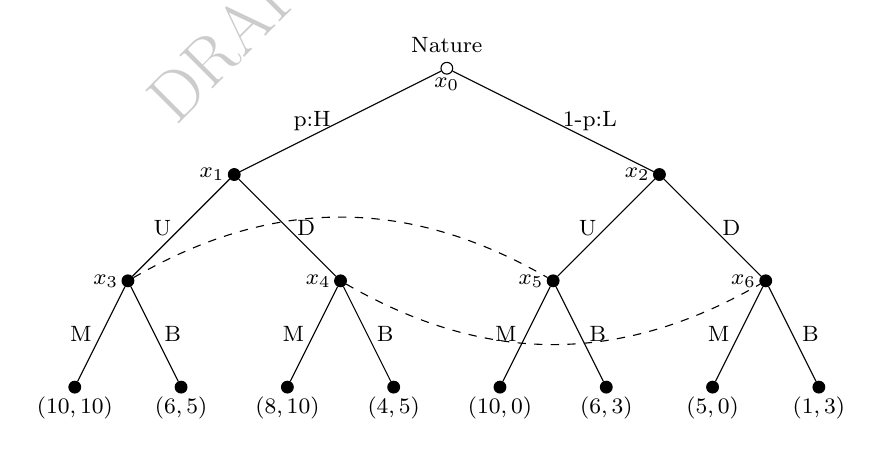
\begin{tikzpicture}[scale=0.9,font=\footnotesize,centered]
			% macro for inputing payoff vectors
			\newcommand{\payoff}[3][below]{\node[#1]at(#2){#3};}
			\newcommand{\assnum}[3][left]{\node[#1]at(#2){#3};}
			% Specify spacing for each level of the tree
			\tikzstyle{level 1}=[level distance=15mm,sibling distance=60mm]
			\tikzstyle{level 2}=[level distance=15mm,sibling distance=30mm]	
			\tikzstyle{level 3}=[level distance=15mm,sibling distance=15mm]	
			
			\node(0)[hollow node,label = above:{Nature}]{}
			child{
				node(0-1)[solid node]{}
				child{
					node(0-1-1)[solid node]{}
					child{
						node(0-1-1-1)[solid node]{}
						edge from parent[draw] node[left]{M}
					}
					child{
						node(0-1-1-2)[solid node]{}
						edge from parent[draw] node[right]{B}
					}
					edge from parent[draw] node[left]{U}
				}
				child{
					node(0-1-2)[solid node]{}
					child{
						node(0-1-2-1)[solid node]{}
						edge from parent[draw] node[left]{M}
					}
					child{
						node(0-1-2-2)[solid node]{}
						edge from parent[draw] node[right]{B}
					}
					edge from parent[draw] node[right]{D}
				}
				edge from parent[draw] node[left]{p:H}
			}
			child{
				node(0-2)[solid node]{}
				child{
					node(0-2-1)[solid node]{}
					child{
						node(0-2-1-1)[solid node]{}
						edge from parent[draw] node[left]{M}
					}
					child{
						node(0-2-1-2)[solid node]{}
						edge from parent[draw] node[right]{B}
					}
					edge from parent[draw] node[left]{U}
				}
				child{
					node(0-2-2)[solid node]{}
					child{
						node(0-2-2-1)[solid node]{}
						edge from parent[draw] node[left]{M}
					}
					child{
						node(0-2-2-2)[solid node]{}
						edge from parent[draw] node[right]{B}
					}
					edge from parent[draw] node[right]{D}
				}
				edge from parent[draw] node[right]{1-p:L}
			}
			;
			
			\assnum[below]{0}{$x_0$}
			\assnum{0-1}{$x_1$}
			\assnum{0-2}{$x_2$}
			\assnum{0-1-1}{$x_3$}
			\assnum{0-1-2}{$x_4$}
			\assnum{0-2-1}{$x_5$}
			\assnum{0-2-2}{$x_6$}

			
			\payoff{0-1-1-1}{$(10,10)$}
			\payoff{0-1-1-2}{$(6,5)$}
			\payoff{0-1-2-1}{$(8,10)$}
			\payoff{0-1-2-2}{$(4,5)$}
			\payoff{0-2-1-1}{$(10,0)$}
			\payoff{0-2-1-2}{$(6,3)$}
			\payoff{0-2-2-1}{$(5,0)$}
			\payoff{0-2-2-2}{$(1,3)$}
			
			\draw[dashed,bend right](0-1-2) to (0-2-2);
			\draw[dashed,bend left](0-1-1) to (0-2-1);
		\end{tikzpicture}
	\end{figure}
\end{document}